% Chapter 12: LTL Model Checking and Fairness
% Sources: Course 89, L18-L19

\chapter{LTL Model Checking and Fairness}
\label{ch:ltl-mc-fairness}

\aside{An LTL formula becomes useful to an engineer only when it can be
checked against a finite model, and a violated formula becomes useful only
when the checker returns a concrete infinite witness.}

Chapter~\ref{ch:ltl} gave LTL its syntax, semantics, and tableau-based
satisfiability machinery.  We now turn that logical language into a model
checking procedure.  The shift is small in notation but decisive in
meaning: instead of asking whether \emph{some} infinite trace satisfies a
formula, we ask whether \emph{all} executions of a finite system satisfy it.
The answer is computed by negating the property, translating the negation
into a B\"uchi automaton, taking the product with the system, and searching
for an accepting lasso.  If such a lasso exists, it is the counterexample.
If it does not, the system satisfies the property.

The lecture material for this chapter has two layers.  First comes the
classical automata-theoretic model checking pipeline.  Then comes the
fairness refinement: justice and compassion are path filters that discard
unrealistic scheduler behaviours before the property is judged.  On a finite
graph, fairness is handled by strongly connected component search, which is
why the practical algorithms look so much like the emptiness test for
B\"uchi automata from Part~I.

% =======================================================================
\section{From a Formula to an Emptiness Problem}
\label{sec:ltl-mc-pipeline}

The key observation behind LTL model checking is simple: a universal
verification question can be turned into an existential search for a bad
behaviour.  Instead of proving that every execution satisfies $\varphi$, we
look for an execution that satisfies $\neg\varphi$.

\begin{definition}[Kripke structure]
\label{def:kripke-structure}
A \emph{Kripke structure} over a set of atomic propositions $AP$ is a tuple
\[
  \mathcal{M} = (Q, I, R, L)
\]
where $Q$ is a finite set of states, $I \subseteq Q$ is the set of initial
states, $R \subseteq Q \times Q$ is a total transition relation, and
$L : Q \to 2^{AP}$ labels each state with the propositions that hold there.
\end{definition}

The LTL model checking problem is:
\[
  \mathcal{M} \models \varphi \quad\text{?}
\]
meaning that every infinite path starting from an initial state of
$\mathcal{M}$ satisfies $\varphi$.

\begin{theorem}[Automata-theoretic model checking]
\label{thm:ltl-mc-automata}
Let $\mathcal{M}$ be a Kripke structure and $\varphi$ an LTL formula.  Then
\[
  \mathcal{M} \models \varphi
  \iff
  L(\mathcal{M}) \cap L(\neg \varphi) = \emptyset
  \iff
  \mathcal{M} \times \mathcal{A}_{\neg\varphi}
  \text{ has no accepting run}
\]
where $\mathcal{A}_{\neg\varphi}$ is a B\"uchi automaton for the negated
formula.
\end{theorem}

\begin{proof}[Idea]
If $\mathcal{M} \not\models \varphi$, then some path of $\mathcal{M}$
satisfies $\neg\varphi$.  The automaton $\mathcal{A}_{\neg\varphi}$ accepts
exactly those paths, so the product has an accepting run.  Conversely, any
accepting run of the product projects to a path of $\mathcal{M}$ that
satisfies $\neg\varphi$.
\end{proof}

\medskip\noindent
\textbf{Why negation helps.}  The universal verification question is hard
only because it quantifies over every behaviour.  By negating the property we
move to an existential problem: find one bad trace.  B\"uchi automata are
already designed to recognise existential infinite witnesses, so this is the
right target representation.

\begin{figure}[ht]
  \centering
  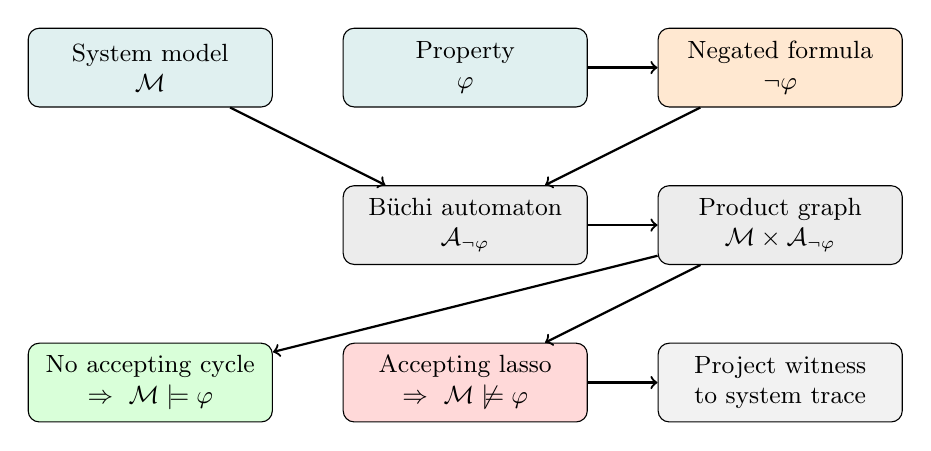
\begin{tikzpicture}[
      box/.style={draw, rounded corners, minimum width=3.1cm,
                  minimum height=1.0cm, align=center, font=\small},
      arr/.style={->, thick}
    ]
    \node[box, fill=teal!12]   (sys)  at (0,0)    {System model\\$\mathcal{M}$};
    \node[box, fill=teal!12]   (phi)  at (4,0)    {Property\\$\varphi$};
    \node[box, fill=orange!18] (nphi) at (8,0)    {Negated formula\\$\neg\varphi$};
    \node[box, fill=gray!15]   (aut)  at (4,-2)   {B\"uchi automaton\\$\mathcal{A}_{\neg\varphi}$};
    \node[box, fill=gray!15]   (prod) at (8,-2)   {Product graph\\$\mathcal{M}\times\mathcal{A}_{\neg\varphi}$};
    \node[box, fill=green!15]  (ok)   at (0,-4)   {No accepting cycle\\$\Rightarrow\ \mathcal{M}\models\varphi$};
    \node[box, fill=red!15]    (bad)  at (4,-4)   {Accepting lasso\\$\Rightarrow\ \mathcal{M}\not\models\varphi$};
    \node[box, fill=gray!10]   (w)    at (8,-4)   {Project witness\\to system trace};

    \draw[arr] (sys) -- (aut);
    \draw[arr] (phi) -- (nphi);
    \draw[arr] (nphi) -- (aut);
    \draw[arr] (aut) -- (prod);
    \draw[arr] (prod) -- (bad);
    \draw[arr] (bad) -- (w);
    \draw[arr] (prod) -- (ok);
  \end{tikzpicture}
  \caption{The LTL model-checking pipeline.  Negate the property, compile
           the negation to a B\"uchi automaton, take the product with the
           system, and search for an accepting cycle.}
  \label{fig:ltl-mc-pipeline}
\end{figure}

\subsection{The product construction}

The product graph keeps track of both the system state and the current
automaton state.

\begin{definition}[Product with a B\"uchi automaton]
Let $\mathcal{M} = (Q, I, R, L)$ and let
\[
  \mathcal{A} = (Q_A, \Sigma, I_A, \Delta, F)
\]
be a B\"uchi automaton over $\Sigma = 2^{AP}$.  The product
$\mathcal{M} \times \mathcal{A}$ has:
\begin{itemize}
  \item states $Q \times Q_A$;
  \item initial states $\{(q,a) \mid q \in I,\ a \in I_A,\ a \text{ is
        compatible with } L(q)\}$;
  \item transitions
        \[
          (q,a) \to (q',a')
          \iff
          (q,q') \in R \text{ and } a' \in \Delta(a, L(q'));
        \]
  \item accepting states $Q \times F$.
\end{itemize}
\end{definition}

The intuition is straightforward.  The system chooses the next concrete
state; the automaton reacts to the label of that state; the product records
both moves at once.  A counterexample is therefore not just a path in the
system, but a path annotated with the automaton states that explain why the
path violates the property.

\begin{example}[A lasso counterexample]
\label{ex:ltl-lasso-counterexample}
Consider the property
\[
  \varphi = \mathbf{G}(r \rightarrow \mathbf{F}g)
\]
over a system where a request $r$ may become true and then remain pending
forever if no grant $g$ occurs.  The negation is the statement that there is
some point after which a request is never followed by a grant.

Suppose the system has a path
\[
  s_0 \to s_1 \to s_1 \to s_1 \to \cdots
\]
where $r$ becomes true in $s_1$ and $g$ never appears again.  The product
with $\mathcal{A}_{\neg\varphi}$ contains a reachable accepting cycle on the
pair corresponding to $s_1$.  The checker reports the witness as the lasso
\[
  s_0 \to s_1 \to (s_1)^\omega.
\]
The finite prefix gets us to the bad region; the cycle shows that we can stay
there forever.
\end{example}

\medskip\noindent
\textbf{Why the witness is a lasso.}  The product graph is finite.  Any
infinite path in a finite graph repeats a state, and once a state repeats we
can separate the path into a finite prefix and a cycle.  That is exactly the
shape of a B\"uchi witness: a finite prefix that reaches an accepting cycle,
followed by that cycle repeated forever.

% =======================================================================
\section{Direct Algorithms and SCC Search}
\label{sec:ltl-mc-direct}

The product construction gives the conceptual answer, but real tools rarely
build the whole product explicitly.  They search it on the fly, because the
product can be enormous even when the original model is small.

\subsection{On-the-fly emptiness checking}

The direct algorithm is the model-checking analogue of the Büchi emptiness
test from Part~I.  It explores the reachable portion of the product graph
and looks for a reachable accepting cycle.

\begin{enumerate}
  \item Start from an initial product state.
  \item Explore successors depth-first, generating product states only when
        they are needed.
  \item When an accepting state is encountered, check whether it can reach
        itself again inside the reachable subgraph.
  \item If it can, record the prefix and the cycle as a lasso counterexample.
\end{enumerate}

This is why the algorithm is often described as \emph{direct}.  The checker
never needs the full product in memory; it only needs enough information to
continue the current search and to reconstruct a witness when one is found.
In practice, this is usually implemented with a depth-first traversal,
sometimes with a nested search for the closing cycle.

\subsection{Strongly connected components}

The graph-theoretic view becomes cleaner if we compress the reachable part of
the product into strongly connected components.

\begin{definition}[Accepting SCC]
An SCC of $\mathcal{M}\times\mathcal{A}_{\neg\varphi}$ is \emph{accepting} if
it is reachable from an initial product state, contains at least one
accepting automaton state, and contains a directed cycle.
\end{definition}

\begin{proposition}[SCC criterion for counterexamples]
The model $\mathcal{M}$ violates $\varphi$ if and only if the reachable part
of $\mathcal{M}\times\mathcal{A}_{\neg\varphi}$ contains an accepting SCC.
\end{proposition}

\begin{proof}[Sketch]
Any accepting run eventually stays inside one SCC, because the product graph
is finite.  If the SCC contains an accepting state, the run visits it
infinitely often, so the SCC yields a lasso.  Conversely, every accepting
lasso obviously sits inside a reachable SCC.
\end{proof}

\medskip\noindent
The SCC criterion is the same structural idea that we used for Büchi
emptiness in Part~I and for LTL satisfiability in Chapter~\ref{ch:ltl}.  The
difference is only where the graph comes from: here it is a product of a
system and an automaton rather than a standalone automaton.

\subsection{Complexity}

\begin{proposition}[Complexity of LTL model checking]
\label{prop:ltl-mc-pspace}
LTL model checking is PSPACE-complete.
\end{proposition}

\begin{proof}[Proof sketch]
The upper bound comes from the on-the-fly algorithm.  A product state can be
represented with one system state and one automaton state, both of which have
polynomial descriptions.  The depth-first search stores only the current
search stack and a bounded amount of local information, so the procedure uses
polynomial space.

The lower bound is the standard PSPACE-hardness of LTL satisfiability, which
embeds into model checking by asking whether a suitable finite model admits a
path satisfying the formula.  In other words, model checking already contains
the same hard infinite-word search problem that appears in satisfiability.
\end{proof}

\medskip\noindent
The practical point is that explicit state counts can still explode
exponentially in the size of the formula, even though the decision problem is
only PSPACE-complete.  That is the usual verification trade-off: the worst
case is hard, but the graph search is structured enough to make many real
instances tractable.

% =======================================================================
\section{Fairness}
\label{sec:ltl-mc-fairness}

Chapter~\ref{ch:reactive-smv} introduced fairness as a way to ignore
unrealistic scheduler behaviours.  Here we use the same idea algorithmically:
fairness is a filter on the paths we are allowed to consider when searching
for a counterexample.

The intuition is easiest to state on paths, and then to translate to SCCs.
Suppose a system has several processes competing for the next transition.  A
path that permanently starves one process is usually not the execution we
mean to reason about.  Fairness says that such paths should not count against
the specification.

\subsection{Justice and compassion revisited}

We restate the two fairness notions at the level of runs.

\begin{definition}[Justice and compassion]
Let $\pi$ be an infinite path.
\begin{itemize}
  \item A \emph{justice} constraint says that if a condition remains enabled
        from some point onward, then the corresponding action must occur
        infinitely often.
  \item A \emph{compassion} constraint says that if a condition occurs
        infinitely often, then the corresponding action must also occur
        infinitely often.
\end{itemize}
\end{definition}

These are exactly the notions previewed in Chapter~\ref{ch:reactive-smv}
under the SMV keywords \texttt{JUSTICE} and \texttt{COMPASSION}.  The
important difference is the level of use: there they were presented as a
modelling device; here they become a constraint on the model-checking search
space.

\medskip\noindent
\textbf{Justice is a continuous obligation.}  If a process is continuously
available, it must not be ignored forever.

\medskip\noindent
\textbf{Compassion is a recurring-obligation rule.}  If a process keeps
showing up, even with gaps, the run must still give it infinitely many
opportunities.

\begin{example}[Producer and consumer]
\label{ex:ltl-fair-producer-consumer}
The producer--consumer system from Chapter~\ref{ch:reactive-smv} is a
standard source of unfair counterexamples.  Without fairness, the scheduler
may keep choosing the producer forever.  The buffer fills up, the consumer
never runs, and the property
\[
  \mathbf{G}\bigl(\texttt{full} \rightarrow \mathbf{F}\,\texttt{free}\bigr)
\]
fails.  The counterexample is a lasso whose cycle is the self-loop that keeps
the producer active.

Under fairness, this run is discarded.  If the consumer is continuously
enabled but never scheduled, justice fails.  If the consumer is enabled only
intermittently, compassion is the relevant constraint.  Either way, the
checker only judges the property on fair paths, so the spurious starvation
witness disappears.
\end{example}

\subsection{The SCC criterion for fairness}

On a finite graph, every infinite path eventually stays inside one SCC.  That
is the point where fairness becomes easy to test.

\begin{definition}[Fair SCC]
Let $\mathcal{J}$ be the set of justice constraints and $\mathcal{C}$ the set
of compassion constraints.  A reachable SCC $S$ of the product graph is
\emph{fair} if:
\begin{itemize}
  \item for every justice set $J \in \mathcal{J}$, we have $S \cap J \neq
        \emptyset$;
  \item for every compassion pair $(C,D) \in \mathcal{C}$, if $S \cap C
        \neq \emptyset$ then $S \cap D \neq \emptyset$.
\end{itemize}
\end{definition}

This criterion is the graph version of the path conditions above.  If an SCC
violates justice, then there is a region of the graph in which the scheduler
can stay forever while starving some enabled activity.  If an SCC violates
compassion, then the recurring trigger can be seen forever while the required
response never appears.  In both cases, the SCC cannot host a fair
counterexample.

\medskip\noindent
The practical algorithm therefore builds an \emph{adequate subgraph}: the
reachable part of the product graph after pruning every SCC that cannot
possibly support a fair run.  Once the pruning is done, the remaining graph
is checked with the usual accepting-cycle search.  The adequate-subgraph idea
does not change the underlying semantics; it simply removes regions that are
provably irrelevant.

\begin{figure}[ht]
  \centering
  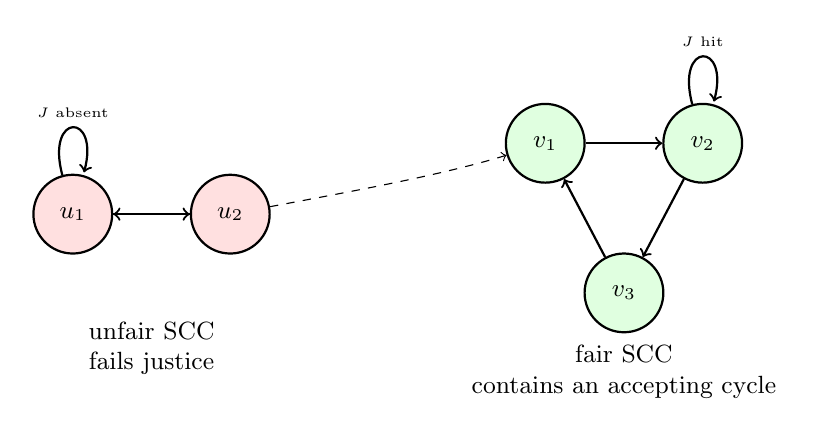
\begin{tikzpicture}[
      st/.style={draw, circle, minimum size=1.0cm, font=\small, thick},
      bad/.style={st, fill=red!12},
      good/.style={st, fill=green!12},
      arr/.style={->, thick}
    ]
    \node[bad]  (b1) at (0,0)   {$u_1$};
    \node[bad]  (b2) at (2,0)   {$u_2$};
    \node[good] (g1) at (6,0.9) {$v_1$};
    \node[good] (g2) at (8,0.9) {$v_2$};
    \node[good] (g3) at (7,-1.0) {$v_3$};

    \node[font=\small, align=center] at (1,-1.7) {unfair SCC\\fails justice};
    \node[font=\small, align=center] at (7,-2.0) {fair SCC\\contains an accepting cycle};

    \draw[arr] (b1) edge[loop above] node[font=\tiny] {$J$ absent} (b1);
    \draw[arr] (b1) -- (b2);
    \draw[arr] (b2) -- (b1);

    \draw[arr] (g1) -- (g2);
    \draw[arr] (g2) -- (g3);
    \draw[arr] (g3) -- (g1);
    \draw[arr] (g2) edge[loop above] node[font=\tiny] {$J$ hit} (g2);

    \draw[->, dashed] (b2) .. controls (3.6,0.3) and (4.7,0.5) .. (g1);
  \end{tikzpicture}
  \caption{Fairness prunes SCCs before the accepting-cycle search.  The left
           SCC is unreachable as a fair witness because it violates justice;
           the right SCC remains as a candidate fair cycle.}
  \label{fig:ltl-fair-scc}
\end{figure}

\subsection{Reading a fair counterexample}

The final witness returned by a fair model checker is still a lasso.  The
difference is that the loop must be fair.  So the reading protocol is:
\begin{enumerate}
  \item follow the prefix until the system enters the bad region;
  \item check that the cycle is reachable inside a fair SCC;
  \item verify that the cycle satisfies the fairness constraints;
  \item project the witness back to the system and explain it in the model's
        vocabulary.
\end{enumerate}

This is exactly why fairness matters in practice.  Without it, a checker may
hand you a technically valid but operationally meaningless lasso.  With it,
the returned witness matches the scheduler assumptions encoded in the model.

% =======================================================================
\section{Summary}
\label{sec:ltl-mc-summary}

\begin{summarybox}
\begin{itemize}[nosep]
  \item LTL model checking asks whether every system execution satisfies a
        property.
  \item The standard reduction negates the property, translates the negation
        to a B\"uchi automaton, and searches the product for an accepting
        cycle.
  \item A counterexample is always a lasso: a finite prefix followed by a
        repeating cycle.
  \item Direct implementations search the implicit product on the fly and use
        SCC structure to find accepting cycles efficiently.
  \item LTL model checking is PSPACE-complete.
  \item Fairness filters unrealistic runs.  Justice and compassion are
        checked by SCC pruning: a reachable SCC is fair only if it meets the
        justice constraints and respects every compassion pair.
\end{itemize}
\end{summarybox}
